\documentclass{beamer}

\usepackage[utf8]{inputenc}

\usepackage{color}
\usepackage{listings}
\usepackage{tikz}
\usepackage{hyperref}

\usetheme{Rochester}
\usecolortheme{beaver}

\lstloadlanguages{[5.2]Lua,C++}
    \lstset{%
        language={[5.2]Lua},
        basicstyle=\ttfamily,
        keywordstyle=\color{blue},
        showstringspaces=false,
        escapechar={§},
        escapeinside=||
    }

\newif\iftransitions
 \transitionstrue


\newif\iffast
 \fasttrue

\title{Howling at the Moon:}
\subtitle{Lua for C++ Programmers}
\author{Andreas Weis}
\institute{BMW AG}
\date{code::dive, November 14, 2017}
%\titlegraphic{
\includegraphics[height=.25\textheight]{resources/cppcon.png}}


\begin{document}

\frame{\titlepage}

\begin{frame}[fragile]
  \frametitle{About me}

  \begin{itemize}
    \setlength\itemsep{1.5em}

    \item \href{https://stackoverflow.com/users/577603/comicsansms}{
\includegraphics[height=.05\textheight]{resources/so-icon.png}} \href{https://github.com/ComicSansMS}{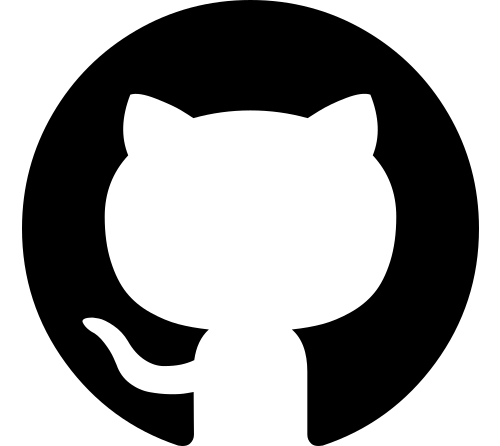
\includegraphics[height=.05\textheight]{resources/github-icon.png}} 
\includegraphics[height=.05\textheight]{resources/slack-icon.png} ComicSansMS

    \item \href{https://twitter.com/DerGhulbus/}{
\includegraphics[height=.05\textheight]{resources/twitter-icon.png} @DerGhulbus}

    \item 
\includegraphics[height=.05\textheight]{resources/meetup-icon.png} Co-organizer of the \href{https://www.meetup.com/MUCplusplus/}{Munich C++ User Group}

    \item Currently working as a Software Architect for BMW 
\includegraphics[height=.1\textheight]{resources/bmw_group.jpg}

  \end{itemize}
\end{frame}

\begin{frame}[fragile]

  \begin{center}
    \href{http://www.lua.org/}{
\includegraphics[height=.8\textheight]{resources/lua-logo.png}}
  \end{center}

\end{frame}

\iffalse
\begin{frame}[fragile]
  \frametitle{Lua}

  \begin{quote}Lua is a powerful, efficient, lightweight, embeddable scripting language.\end{quote}

  \pause

  \begin{itemize}
    \item Powerful
    \item Efficient
    \item Lightweight
    \item Embeddable
  \end{itemize}

  \begin{itemize}
  \item Powerful - First-class functions w/ full lexical scoping; Support for OOP paradigms; Metaprogramming; Reflection
  \item Efficient - Performance better or on par with other scripting languages; Even better with LuaJIT
  \item Lightweight - Small binaries; Only one type of complex data structure; Great expressiveness through few, orthogonal constructs
  \item Embeddable - Simple and lean API; \texttt{main()} belongs to the enclosing program
  \end{itemize}

\end{frame}
\fi

\begin{frame}[fragile]

  \frametitle{A little bit of history\ldots}
  
  \begin{center}
    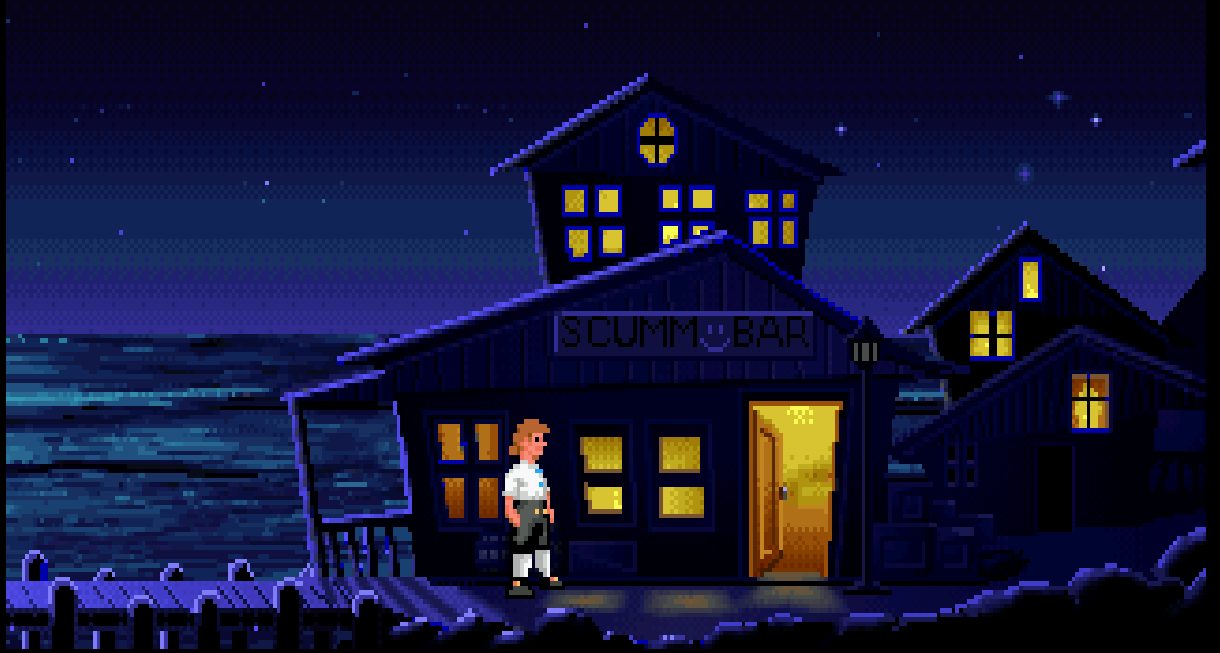
\includegraphics[height=.75\textheight]{resources/scumm_bar.png}
  \end{center}
  
  \iftransitions \pause \fi
  {\scriptsize The Secret of Monkey Island, Lucasfilm Games, 1990}
\end{frame}

\begin{frame}[fragile]

  \begin{center}
    
\includegraphics[height=.75\textheight]{resources/mi_lua_bar.jpg}
  \end{center}

  {\scriptsize Escape from Monkey Island, LucasArts, 2000}
\end{frame}


\begin{frame}
  \frametitle{Lua in the wild}

  \begin{columns}[t]
    \column{.5\textwidth}
    \centering
    
\includegraphics[height=3.5cm]{resources/wow_raidui.png}\\
    
\includegraphics[height=3.5cm]{resources/love2d.png}
    \column{.5\textwidth}
    \centering
    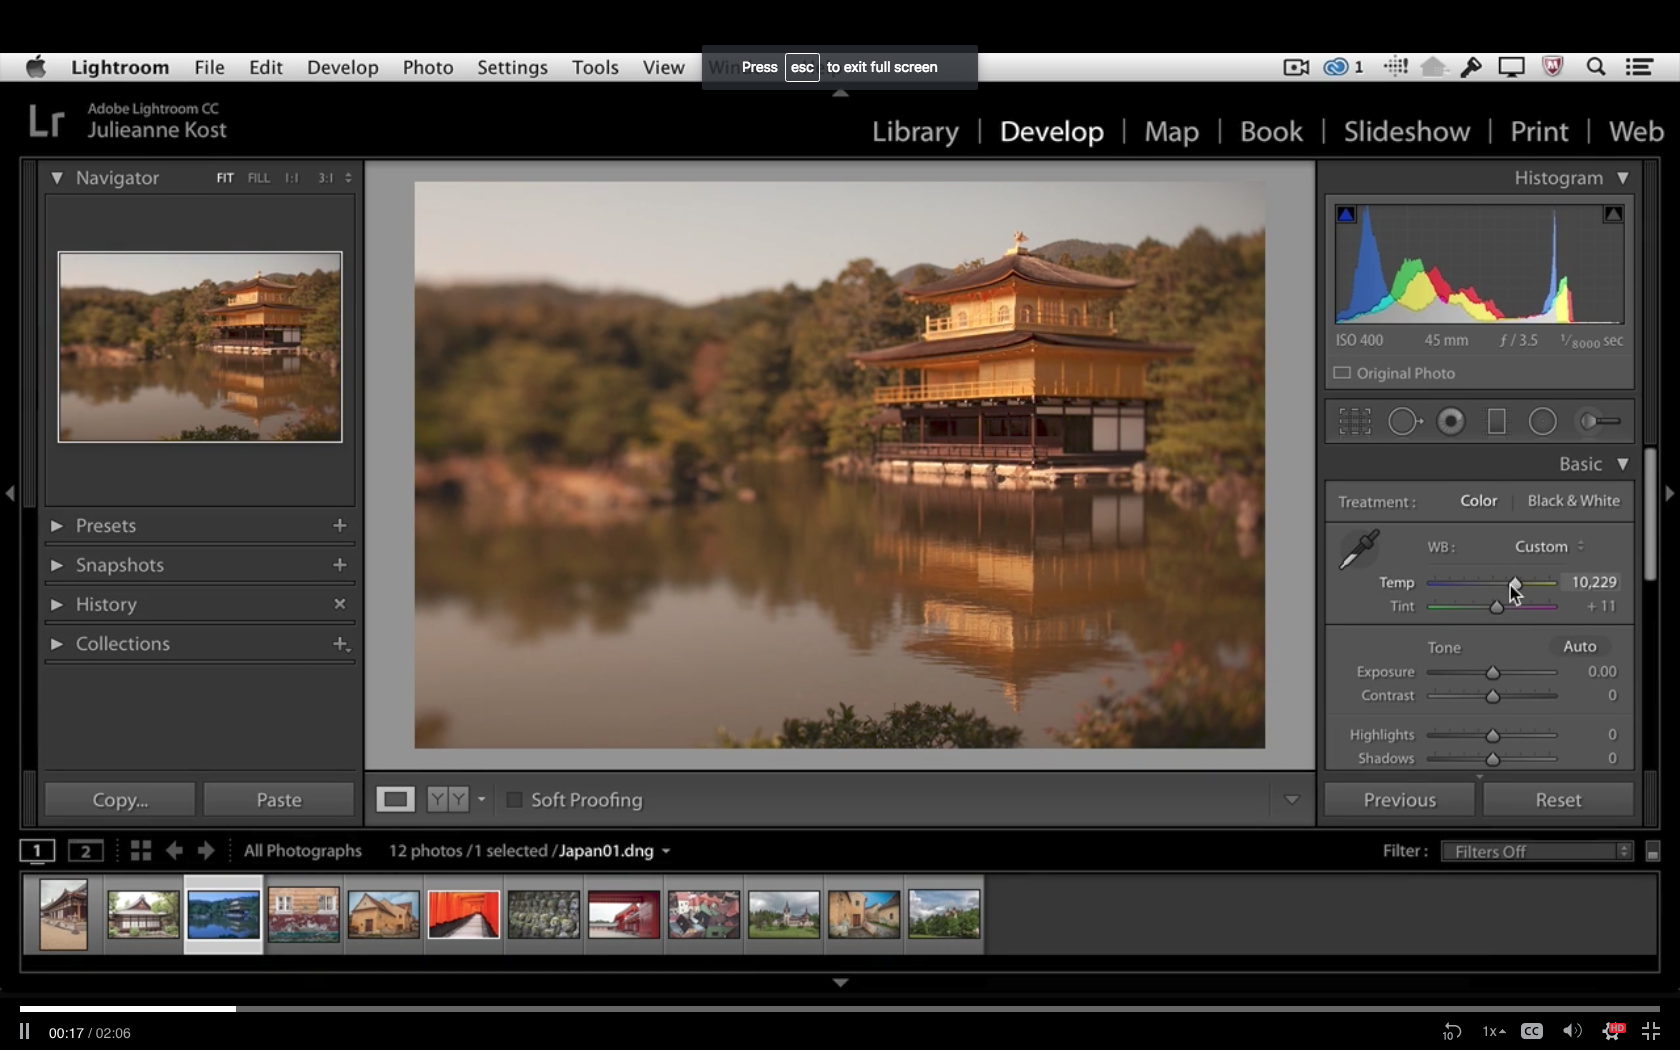
\includegraphics[height=3.5cm]{resources/lightroom.png}\\
    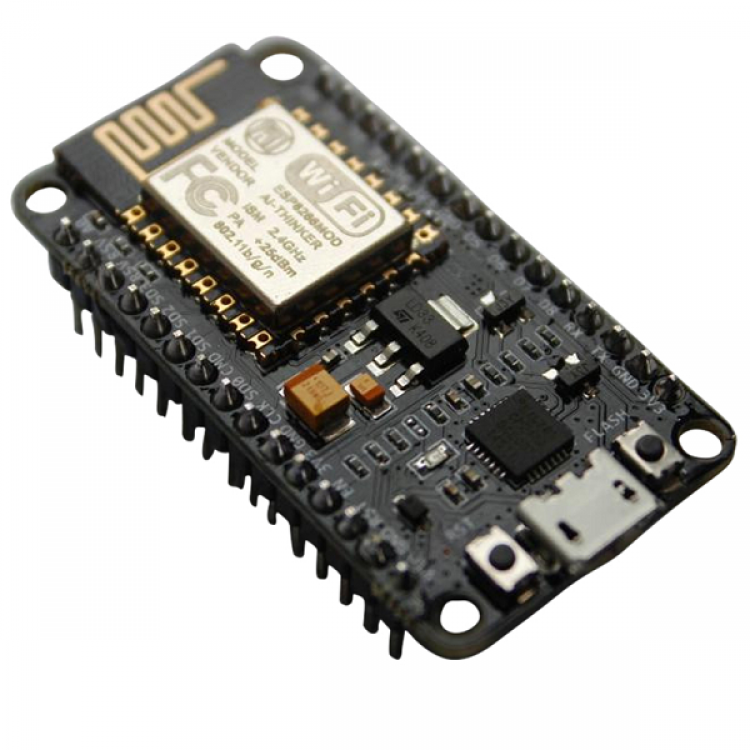
\includegraphics[height=3.5cm]{resources/nodemcu.png}
  \end{columns}

\end{frame}

\iffalse
\begin{frame}
  \frametitle{Why bother with Lua?}

  Lua is \emph{small}.

  (In a good way)

  The interpreter fits into L2 cache of a modern desktop x86.

  \begin{itemize}
  \item The whole language fits in your head.
  \item No swapping required.
  \end{itemize}
\end{frame}
\fi

\begin{frame}
  \frametitle{Lua is small}
  \begin{columns}
    \column{0.4\linewidth}
    \includegraphics[height=.9\textheight]{resources/syntax.pdf}
    \column{0.6\linewidth}
    \begin{itemize}
    \item Compiled binary is $<180$KB
    \item Reference Manual 82 A4 pages
%    \item 120 C API functions
    \item 8 basic data types
    \item Batteries not included!
    \end{itemize}
  \end{columns}
\end{frame}

\begin{frame}
  \frametitle{The whole language fits into your head}

  \iftransitions \pause \fi
  \begin{center}
    \includegraphics[height=.9\textheight]{resources/talosians_cpp.jpg}
  \end{center}
\end{frame}

\begin{frame}

  \frametitle{Disclaimer}

  This talk is trying too hard to be clever.

  Keep simple things simple.
\end{frame}

\begin{frame}[fragile]
  \frametitle{Hello World!}

  \begin{lstlisting}
print("Hello World!");
  \end{lstlisting}
\end{frame}

\iffast
\begin{frame}[fragile]

  \frametitle{Functions}

  \begin{lstlisting}
function f(a1, a2, a3)
  -- implementation
  -- [...]
  return r1, r2, r3;
end
  \end{lstlisting}

  \iftransitions \pause \fi
  \begin{semiverbatim}
y1, y2, y3 = f(x1, x2, x3);  \iftransitions \pause \fi
y1 = f(x1, x2, x3);  \iftransitions \pause \fi
f();
  \end{semiverbatim}
\end{frame}
\fi

\begin{frame}[fragile]
  \frametitle{All functions are lambdas}

  \begin{lstlisting}
function f(a1, a2, a3)
  -- [...]
end
  \end{lstlisting}

   \iftransitions \pause \fi

  is just syntax sugar for

  \begin{lstlisting}
f = function(a1, a2, a3)
  -- [...]
end
  \end{lstlisting}

  \iftransitions \pause \fi
  Functions are true first-class values in Lua.
\end{frame}

\begin{frame}[fragile]
  \frametitle{Replacing functions is trivial}

  \begin{lstlisting}
print("Vanilla print");
  \end{lstlisting}
      \iftransitions \pause \fi
    \begin{lstlisting}
print = function(...)
    -- my_print implementation
    -- [...]
  end;
print("My print");
\end{lstlisting}  
\end{frame}

\begin{frame}[fragile]

  \frametitle{Function Hooking -- Counting \texttt{print} calls}

  \begin{lstlisting}
count = 0;
old_print = print;
print = function(...)
    count = count + 1;
    old_print(...);
  end;
  \end{lstlisting}

\end{frame}


\begin{frame}[fragile]

  \frametitle{Capturing state with function closures}

  Instead of explicit Lambda captures, Lua has full lexical scoping.
  \iftransitions \pause \fi

\iftransitions
  \setbeamercolor{alerted text}{fg=red}
  \setbeamerfont{alerted text}{series=\bfseries,family=\ttfamily}
  \begin{semiverbatim}
\uncover<2->{\alert<0>{{\color{blue}function} enable_counting()}}
\uncover<2->{\alert<0>{  {\color{blue}local} count = 0;}}
\uncover<2->{\alert<0>{  {\color{blue}local} old_print = {\color{blue}print};}}
\uncover<3->{\alert<3>{  {\color{blue}print} = {\color{blue}function}(...)}}
\uncover<3->{\alert<3>{      count = count + 1;}}
\uncover<3->{\alert<3>{      old_print(...);}}
\uncover<3->{\alert<3>{    {\color{blue}end};}}

\uncover<4->{\alert<4>{  {\color{blue}return function}() {\color{blue}return} count; {\color{blue}end};}}
\uncover<2->{\alert<0>{{\color{blue}end}}}

  \end{semiverbatim}
\else
  \begin{lstlisting}
function enable_counting()
  local count = 0;
  local old_print = print;
  print = function(...)
      count = count + 1;
      old_print(...);
    end;

  return function() return count; end;
end
  \end{lstlisting}
\fi

  \iftransitions \uncover<5->{\fi
  Read \texttt{function} as closure construction.
  \iftransitions }\fi
\end{frame}


\begin{frame}[fragile]
  \frametitle{Tables}

  The only complex data structure in the language.

  \begin{lstlisting}
local t = {};
  \end{lstlisting}
  \iftransitions \pause \fi
  \begin{lstlisting}
local array = { 5, 4, 3, 2, 1 };
assert(array[2] == 4);   -- indices are 1-based
  \end{lstlisting}
  \iftransitions \pause \fi
  \begin{lstlisting}
local dict = { the_answer = 42 };
assert(dict["the_answer"] == 42);
  \end{lstlisting}
  \iftransitions \pause \fi

  Tables can use any type of values as keys or values.

  \begin{lstlisting}
dict[print] = "function as key";
  \end{lstlisting}
\end{frame}


\begin{frame}[fragile]
  \frametitle{Tables (contd.)}

  \iffalse
  \begin{lstlisting}
local set = {};
set["foo"] = true;
set["bar"] = true;
  \end{lstlisting}

  \iftransitions \pause \fi
  \fi
  Tables have reference semantics:

  \begin{lstlisting}
local list = { value = "foo", next = nil };
list.next = { value = "bar", next = nil  };
  \end{lstlisting}

  \iftransitions \pause \fi

  Read \texttt{\{\}} as table construction.
\end{frame}



\begin{frame}[fragile]

  \frametitle{Records}

  \begin{lstlisting}
local complex = { real = 42.0, imag = 0.0 };
complex["real"] = 42.0;
complex.real = 42.0;
  \end{lstlisting}
    \iftransitions \pause \fi
  \begin{lstlisting}
function fconjugate(c)
  c.imag = 0.0 - c.imag;
end
  \end{lstlisting}
  \iftransitions \pause \fi
  \begin{lstlisting}
complex.conjugate = fconjugate;
complex.conjugate(complex);
  \end{lstlisting}
  \iftransitions \pause \fi
  \begin{lstlisting}
complex:conjugate();
  \end{lstlisting}

\end{frame}

\begin{frame}[fragile]
  \frametitle{Object Construction}

  \begin{lstlisting}
function build_complex(r, i)
  return { real = r, imag = i };
end

local c1 = build_complex(1, 0);
local c2 = build_complex(0, 1);
  \end{lstlisting}
  \iftransitions \pause \fi
  \begin{lstlisting}
local sum = c1 + c2; -- ???
  \end{lstlisting}
\end{frame}


\begin{frame}[fragile]
  \frametitle{Metatables - Tables describing object properties}

  \begin{lstlisting}
local mt = {};
mt.__add = function(c1, c2)
    return build_complex(c1.real + c2.real,
                         c1.imag + c2.imag);
  end;
  \end{lstlisting}
  \iftransitions \pause \fi
  \begin{lstlisting}
function build_complex(r,i)
  local ret = {real = r, imag = i};
  setmetatable(ret, mt);
  return ret;
end
  \end{lstlisting}
\end{frame}

\iffast
\begin{frame}[fragile]
  \frametitle{Metatables on non-table values}

  \begin{lstlisting}
local str = "The quick brown fox";
assert(str:find("quick") == 5)
  \end{lstlisting}

  \iftransitions \pause \fi
  
  Metatables are extensible: Functions can add their own semantics for non-standard fields.
\end{frame}
\fi

\iftransitions

\begin{frame}[fragile]
  \frametitle{Encapsulation}
  \setbeamercolor{alerted text}{fg=red}
  \setbeamerfont{alerted text}{series=\bfseries,family=\ttfamily}
  \begin{semiverbatim}
\uncover<1->{\alert<0>{{\color{blue}function} build_date(y, m, d)}}
\uncover<3->{\alert<3>{  assert(validDate(y, m, d))}}
\uncover<3->{\alert<3>{  {\color{blue}local} lself = \{ y=y, m=m, d=d \}}}
\uncover<3->{\alert<3>{}}
\uncover<4->{\alert<4>{  {\color{blue}local} lget_day = {\color{blue}function}() {\color{blue}return} lself.d {\color{blue}end}}}
\uncover<5->{\alert<5>{  {\color{blue}local} lset_day = {\color{blue}function}(nd)}}
\uncover<5->{\alert<5>{      assert(validDate(lself.y, lself.m, nd))}}
\uncover<5->{\alert<5>{      lself.d = nd}}
\uncover<5->{\alert<5>{    {\color{blue}end}}}
\uncover<5->{\alert<5>{}}
\uncover<2->{\alert<2>{  {\color{blue}return} \{}}
\uncover<2->{\alert<2>{    set_day = lset_day,}}
\uncover<2->{\alert<2>{    get_day = lget_day}}
\uncover<2->{\alert<2>{  \}}}
\uncover<1->{\alert<0>{\color{blue}end}}
  \end{semiverbatim}
\uncover<6->{}
\end{frame}

\else

\begin{frame}[fragile]
  \frametitle{Encapsulation}

  \begin{lstlisting}
function build_date(y, m, d)
  assert(validDate(y, m, d))
  local lself = { y=y, m=m, d=d }

  local lget_day = function() return lself.d end
  local lset_day = function(nd)
      assert(validDate(lself.y, lself.m, nd))
      lself.d = nd
    end

  return {
    set_day = lset_day,
    get_day = lget_day
  }
  \end{lstlisting}
\end{frame}

\fi


\begin{frame}[fragile]
  \frametitle{Reflection}

  All data structures are tables. Inspecting the fields of the table reveals everything we need to know about the type.

  \begin{lstlisting}
function is_complex(c)
  return type(c) == "table" and
         c.real and c.imag;    
end
  \end{lstlisting}
  \iftransitions \pause \fi
  \begin{lstlisting}
local tuple = {};
for k,v in pairs(t) do
  tuple[#tuple + 1] = v;
end
  \end{lstlisting}
\end{frame}


\begin{frame}[fragile]

  \frametitle{The environment}

  But what about global variables?
  \iftransitions \pause \fi
  \begin{lstlisting}
for k in pairs(_G) do
  print(k);
end
  \end{lstlisting}

%  What about local variables?
%  Sorry, no.
\end{frame}

\iffast
\begin{frame}[fragile]

  \frametitle{Back to function hooking}

  \iftransitions
  \setbeamercolor{alerted text}{fg=red}
  \setbeamerfont{alerted text}{series=\bfseries,family=\ttfamily}
  \begin{semiverbatim}
\uncover<1->{\alert<0>{{\color{blue}function} enable_counting(fname)}}
\uncover<2->{\alert<2>{  {\color{blue}local} count = 0;}}
\uncover<2->{\alert<2>{  {\color{blue}local} old_func = {\color{blue}_G}[fname];}}
\uncover<3->{\alert<3>{  {\color{blue}_G}[fname] = {\color{blue}function}(...)}}
\uncover<3->{\alert<3>{      count = count + 1;}}
\uncover<3->{\alert<3>{      {\color{blue}return} old_func(...);}}
\uncover<3->{\alert<3>{    {\color{blue}end};}}
\uncover<3->{\alert<3>{  {\color{blue}return function}() {\color{blue}return} count; {\color{blue}end};}}
\uncover<1->{\alert<0>{{\color{blue}end}}}

\uncover<1->{\alert<0>{{\color{blue}local} c = enable_counting("print");}}
\uncover<1->{\alert<0>{c();  -- retrieve count}}

  \end{semiverbatim}
  \else
  \begin{lstlisting}
function enable_counting(fname)
  local count = 0;
  local old_func = _G[fname];
  _G[fname] = function(...)
      count = count + 1;
      return old_func(...);
    end;
  return function() return count; end;
end

local c = enable_counting("print");
c();  -- retrieve count
  \end{lstlisting}
  \fi

\end{frame}
\fi


\begin{frame}[fragile]

  \frametitle{Constraining the environment}

  \begin{lstlisting}
local foobar;
-- [...]
fobar = do_stuff();
  \end{lstlisting}
  \iftransitions \pause \fi
  Remember: \texttt{\_G} is just a table.
  \iftransitions \pause \fi
  \begin{lstlisting}
setmetatable(_G,
  { __newindex = function(_, name)
      print(name .. " was not declared!");
    end
  });
  \end{lstlisting}
  
\end{frame}


\begin{frame}[fragile]

  \frametitle{Integration with C++}

  \iftransitions \pause \fi

  It's embedded --- \texttt{main()} belongs to the enclosing program.

  \iftransitions
  \setbeamercolor{alerted text}{fg=red}
  \setbeamerfont{alerted text}{series=\bfseries,family=\ttfamily}
  \begin{semiverbatim}
\uncover<2->{\alert<0>{{\color{blue}int} main() \{}}

\uncover<3->{\alert<0>{  lua_State* l = luaL_newstate();}}

\uncover<4->{\alert<0>{  luaL_dostring(l, R"(}}
\uncover<4->{\alert<0>{      print("Hello World!");}}
\uncover<4->{\alert<0>{    )" );}}
      
\uncover<3->{\alert<0>{  lua_close(l);}}
\uncover<2->{\alert<0>{\}}}
  \end{semiverbatim}
  \else
  \begin{lstlisting}[language={C++}]
int main() {

  lua_State* l = luaL_newstate();

  luaL_dostring(l, R"(
      print("Hello World!");
    )" );
      
  lua_close(l);
}
  \end{lstlisting}
  \fi
  
  Lua API is prefixed \texttt{lua\_}
  
  Auxiliary library is prefixed \texttt{luaL\_}
  
\end{frame}


\begin{frame}[fragile]
  \frametitle{Exposing C functions to Lua}

  \begin{lstlisting}[language={C++}]
int my_function(lua_State* l) {
      // [...]
}
  \end{lstlisting}
  
\end{frame}

\begin{frame}

  \frametitle{The Stack - The needle's eye}

  \begin{center}
    
\includegraphics[height=.9\textheight]{resources/needle.png}
  \end{center}

\end{frame}

\iffalse
  \begin{itemize}
  \item A stack of Lua values.
  \item The only way of getting values in or out of the VM.
  \item API functions consume Lua value arguments from the stack.
  \item Function calls exchange arguments and return values over the stack.
  \item The stack has shared ownership of its values.

  \item This is \emph{not} the call stack!
  \end{itemize}
\fi

\begin{frame}[fragile]
  \frametitle{Pushing values on the stack}

  \begin{lstlisting}[language={C++}]
void push(lua_State* l, lua_Number n) {
  lua_pushnumber(l, n);
}

void push(lua_State* l, char const* s) {
  lua_pushstring(l, str);
}
  \end{lstlisting}
  \iftransitions \pause \fi
  \begin{lstlisting}[language={C++}]
template<typename... Ts>
void pushargs(lua_State* l, Ts... args) {
    ( push(l, args), ... );
}
  \end{lstlisting}
\end{frame}

\begin{frame}[fragile]
  \frametitle{Pushing values on the stack (2)}

  \begin{lstlisting}[language={C++}]
template<typename... Ts>
void pushargs(lua_State* l, Ts... args) {
    auto t = boost::hana::make_tuple(args...);
    boost::hana::for_each(t,
      [l](auto&& v) { push(l, v); });
}
  \end{lstlisting}
\end{frame}

\begin{frame}[fragile]
  \frametitle{Pushing values on the stack (3)}

  \begin{lstlisting}[language={C++}]
template<typename... Ts>
void pushargs(lua_State* l, Ts... args) {
  auto t = std::make_tuple(args...);
  push_helper(l, t,
    std::make_index_sequence<sizeof...(Ts)>());
}

template<typename... Ts, std::size_t... Is>
void push_helper(lua_State* l,
                 std::tuple<Ts...> const& t,
                 std::index_sequence<Is...>) {
    using expander = int [];
    (void) expander { 0,
      (push(l, std::get<Is>(t)), 0)... };
}
  \end{lstlisting}
\end{frame}


\begin{frame}[fragile]

  \frametitle{Getting values from the stack}

  \begin{lstlisting}[language={C++}]
??? getValueFromStack(lua_State* l, int idx)
{
  switch(lua_type(l, idx)) {
    case LUA_TNUMBER:
      return Number(lua_tonumber(l, idx));
    case LUA_TSTRING:
      return String(lua_tostring(l, idx));  
    // [...]  
  }
}
  \end{lstlisting}

\end{frame}


\begin{frame}[fragile]
  \frametitle{Representing values}

  \begin{lstlisting}[language={C++}]
enum class Type;
    
class Number { Type type() const; };
class String { Type type() const; };
// [...]
  \end{lstlisting}
    \iftransitions \pause \fi
  \begin{lstlisting}
using Value =
  std::variant<Number, String /*, [...] */>;
  \end{lstlisting}
  \iftransitions \pause \fi
  \begin{lstlisting}
Type getType(Value const& v) {
  return std::visit(
    [](auto x) { return x.type(); },
    v);  
}
  \end{lstlisting}
\end{frame}

\iffast
\begin{frame}[fragile]
  \frametitle{Representing values - Sean Parent style}

  \begin{lstlisting}[language={C++}]
struct Concept {
  virtual ~Concept() = default;
  virtual Type type() const = 0;
};
  \end{lstlisting}
  \iftransitions \pause \fi
  \begin{lstlisting}
template<typename T>
struct Model : Concept {
  Model(T x): v(x) {}  
    
  Type type() const override {
      return v.type();
  }
  T v;
};
    ...
  \end{lstlisting}
\end{frame}
\begin{frame}[fragile]
  \frametitle{Representing values - Sean Parent style (contd.)}
  \iftransitions
  \setbeamercolor{alerted text}{fg=red}
  \setbeamerfont{alerted text}{series=\bfseries,family=\ttfamily}
  \begin{semiverbatim}
\uncover<1->{\alert<0>{    ...}}
      
\uncover<1->{\alert<0>{{\color{blue}class} Value \{}}
\uncover<2->{\alert<2>{  std::unique_ptr<Concept> c;}}
\uncover<2->{\alert<2>{{\color{blue}public}:}}
\uncover<3->{\alert<3>{  {\color{blue}template}<{\color{blue}typename} T>}}
\uncover<3->{\alert<3>{  Value(T v)}}
\uncover<3->{\alert<3>{  : c(std::make_unique<Model<T>>(v))}}
\uncover<3->{\alert<3>{  \{\}}}

\uncover<4->{\alert<4>{  Type type() {\color{blue}const} \{ {\color{blue}return} c->type(); \}}}
\uncover<1->{\alert<0>{\};}}
    
  \end{semiverbatim}
  \else
  \begin{lstlisting}[language={C++}]
    ...
      
class Value {
  std::unique_ptr<Concept> c;
public:
  template<typename T>
  Value(T v)
  : c(std::make_unique<Model<T>>(v))
  {}

  Type type() const { return c->type(); }
};
  \end{lstlisting}
  \fi
\end{frame}
\fi


\begin{frame}[fragile]
  \frametitle{Calling functions}

  \iftransitions
  \setbeamercolor{alerted text}{fg=red}
  \setbeamerfont{alerted text}{series=\bfseries,family=\ttfamily}
  \begin{semiverbatim}
\uncover<3->{\alert<3>{{\color{blue}template}<{\color{blue}typename}... Ts>}}
\uncover<5->{\alert<5>{std::vector<Value>}}\uncover<1->{\alert<0>{ call(}}
\uncover<1->{\alert<0>{    lua_State* l,}}
\uncover<2->{\alert<2>{    {\color{blue}char const}* func,}}
\uncover<3->{\alert<3>{    Ts... args}}\uncover<1->{\alert<0>{)}}
\uncover<1->{\alert<0>{\{}}
\uncover<2->{\alert<2>{  lua_getglobal(l, func);}}
\uncover<3->{\alert<3>{  pushargs(l, args...);}}
\uncover<4->{\alert<4>{  lua_call(l, {\color{blue}sizeof}...(Ts),}}
\uncover<4->{\alert<4>{           LUA_MULTRET, 0);}}
\uncover<5->{\alert<5>{  {\color{blue}return} getValuesFromStack(l);  }}
\uncover<1->{\alert<0>{\}}}

\uncover<6->{\alert<6>{call(l, "print", 42, "Hello World");}}
\uncover<6->{\alert<6>{  // -> 42.0   Hello World}}
  \end{semiverbatim}
  \else
  \begin{lstlisting}[language={C++}]
template<typename... Ts>
std::vector<Value> call(
    lua_State* l,
    char const* func,
    Ts... args)
{
  lua_getglobal(l, func);
  pushargs(l, args...);
  lua_call(l, sizeof...(Ts),
           LUA_MULTRET, 0);
  return getValuesFromStack(l);  
}

call(l, "print", 42, "Hello World");
  // -> 42.0   Hello World
  \end{lstlisting}
  \fi
\end{frame}


\begin{frame}[fragile]
  \frametitle{Constraining functions}

  \begin{lstlisting}[language={C++}]
template<typename... Ts>
std::vector<Value> call(lua_State*,
  char const*,
  Ts...);
  \end{lstlisting}
  \iftransitions \pause \fi
  \begin{lstlisting}[language={C++}]
std::array<Value, 2> call(lua_State*,
  char const*,
  Value, Value);
  \end{lstlisting}
  \iftransitions \pause \fi
  \begin{lstlisting}[language={C++}]
std::tuple<Number, String> call(lua_State*,
  char const*,
  Number, Number);
  \end{lstlisting}

\end{frame}


\begin{frame}[fragile]
  \frametitle{Sol 2 - An efficient binding library for C++\footnote{\href{https://github.com/ThePhD/sol2}{https://github.com/ThePhD/sol2}}}
  
  
  \begin{lstlisting}[language={C++}]
#include <sol.hpp>
  \end{lstlisting}
  \iftransitions \pause \fi
  \begin{lstlisting}[language={C++}]
lua_state* l;
sol::state_view sv(l);
  \end{lstlisting}
  \iftransitions \pause \fi
  \begin{lstlisting}[language={C++}]
sol::function print_lua = sv["print"];
print_lua(42, "Hello World");
  \end{lstlisting}
\end{frame}


\begin{frame}[fragile]
  \frametitle{Exposing C++ to Lua with Sol 2}

  \begin{lstlisting}[language={C++}]
auto some_func =
  [](int a, int b,
     std::string str,
     sol::object v)
  {
    return std::make_tuple(
               a+b, str.length(),
               v.as<sol::table>()[1]);
  };
  \end{lstlisting}
  \iftransitions \pause \fi

  \begin{lstlisting}[language={C++}]
sv["some_func"] = some_func;
sv.script(R"(
    print(some_func(1, 2, "foo", {3}))
  )");   // -> 3    3    3  
  \end{lstlisting}
\end{frame}


\begin{frame}[fragile]

  \frametitle{From C++ to Lua and back}

  \begin{lstlisting}[language={C++}]
sol::table tab(sv, sol::create);
tab[1] = 3;

auto [a, b, c] =
  sv["some_func"](1, 2, "foo", tab);
  \end{lstlisting}
\end{frame}


\begin{frame}
  \frametitle{Wrapping up}

  \begin{quote}Lua is a powerful, efficient, lightweight, embeddable scripting language.\end{quote}
\end{frame}

\begin{frame}
  \frametitle{Literature}

  \begin{itemize}
  \item \href{https://www.lua.org/manual/5.3/}{Lua 5.3 Reference Manual}
  \item \href{https://www.lua.org/pil/}{Programming in Lua (4th Ed., 2016)}
  \item \href{https://www.lua.org/doc/hopl.pdf}{The evolution of Lua (ACM HOPL 2007)}
  \item \href{https://dl.acm.org/citation.cfm?id=1983083}{Passing a language through the eye of a needle (2011)}
  \item \href{https://www.lua.org/wshop16.html\#ThePhD}{A Sun For the Moon - A Zero-Overhead Lua Abstraction using C++ (Lua Workshop 2016)}
  \item \href{https://www.lua.org/docs.html}{https://www.lua.org/docs.html}
  \end{itemize}

  \begin{itemize}
  \item \href{http://www.drdobbs.com/open-source/lua-an-extensible-embedded-language/184410014}{Dr. Dobb's - Lua: An Extensible Embedded Language (1996)}
  %\item \href{http://sol2.readthedocs.io/en/latest/index.html}{Sol2 Documentation}
  \end{itemize}
\end{frame}

\begin{frame}
  \frametitle{Thanks for your attention.}
\end{frame}


\end{document}
